%!TEX root = ../../super_main.tex

\section{Customer Interaction}

\todo[inline]{Skriv at web-delen er et ekspertsystem og konsekvenserne af dette}

\todo[inline]{MÅSKE: Indsæt de mockups vi har lavet af web-delen}

\todo[inline]{skriv at screenshot er lavet på dev, men hvis folk vil ind og se den bedste side evar skal de ind på prod}
Interactions with the server side application is only be available to customers. They may interact the in two ways, depending on their intent. If customers wish to create new campaigns that customers may contribute to, they may utilize a graphical user interface. 

\todo[inline]{Skriv at URLen i alle screenshots er ``forkert'', og skriv at hvis folk vil besøge den, og oprette campaigns osv, så er den tilgængelig på www.x.dk/data}

\todo[inline]{Beskriv \tabref{tab:browser_routes} i introduktionen }

\begin{table}[!htbp]
    \centering
    \begin{tabular}{|l|l|} 
        \hline
        \textbf{Type} & \textbf{URL}                            \\ \hline 
        \mono{GET}    & \mono{campaigns}                        \\ \hline 
        \mono{POST}   & \mono{campaigns}                        \\ \hline 
        \mono{GET}    & \mono{campaigns/create}                 \\ \hline 
        \mono{GET}    & \mono{campaigns/\{campaign\}}           \\ \hline 
        \mono{GET}    & \mono{campaigns/\{campaign\}/snapshots} \\ \hline 
        \mono{GET}    & \mono{home}                             \\ \hline 
        \mono{POST}   & \mono{login}                            \\ \hline 
        \mono{GET}    & \mono{login}                            \\ \hline 
        \mono{GET}    & \mono{logout}                           \\ \hline 
        \mono{POST}   & \mono{password/email}                   \\ \hline 
        \mono{POST}   & \mono{password/reset}                   \\ \hline 
        \mono{GET}    & \mono{password/reset/\{token?\}}        \\ \hline 
        \mono{POST}   & \mono{register}                         \\ \hline 
        \mono{GET}    & \mono{register}                         \\ \hline 
    \end{tabular}
    \caption{The routes that the is used on the website.}
    \label{tab:browser_routes}
\end{table}

% Welcome not logged in
\begin{figure}[!htbp]
\centering
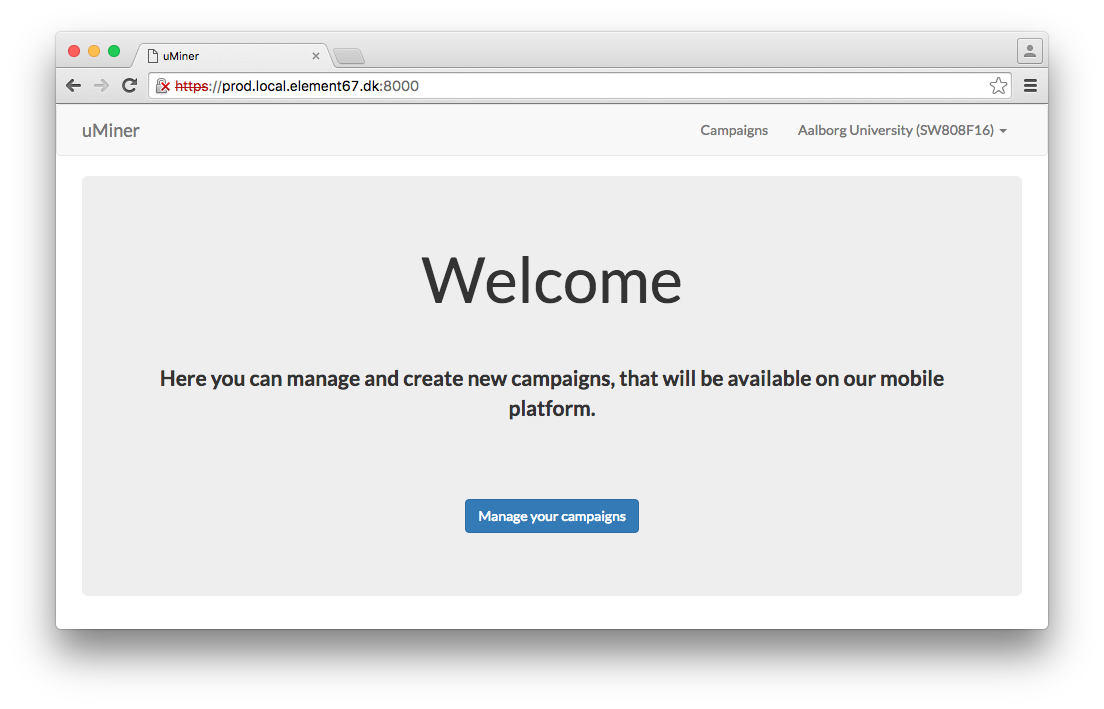
\includegraphics[width=\linewidth]{user_interfaces/web/web_welcome}
\caption{Welcome page.}
\label{fig:web_welcome}
\end{figure}
\FloatBarrier

\subsection{Registration and Logging In}

% Register
\begin{figure}[!htbp]
\centering
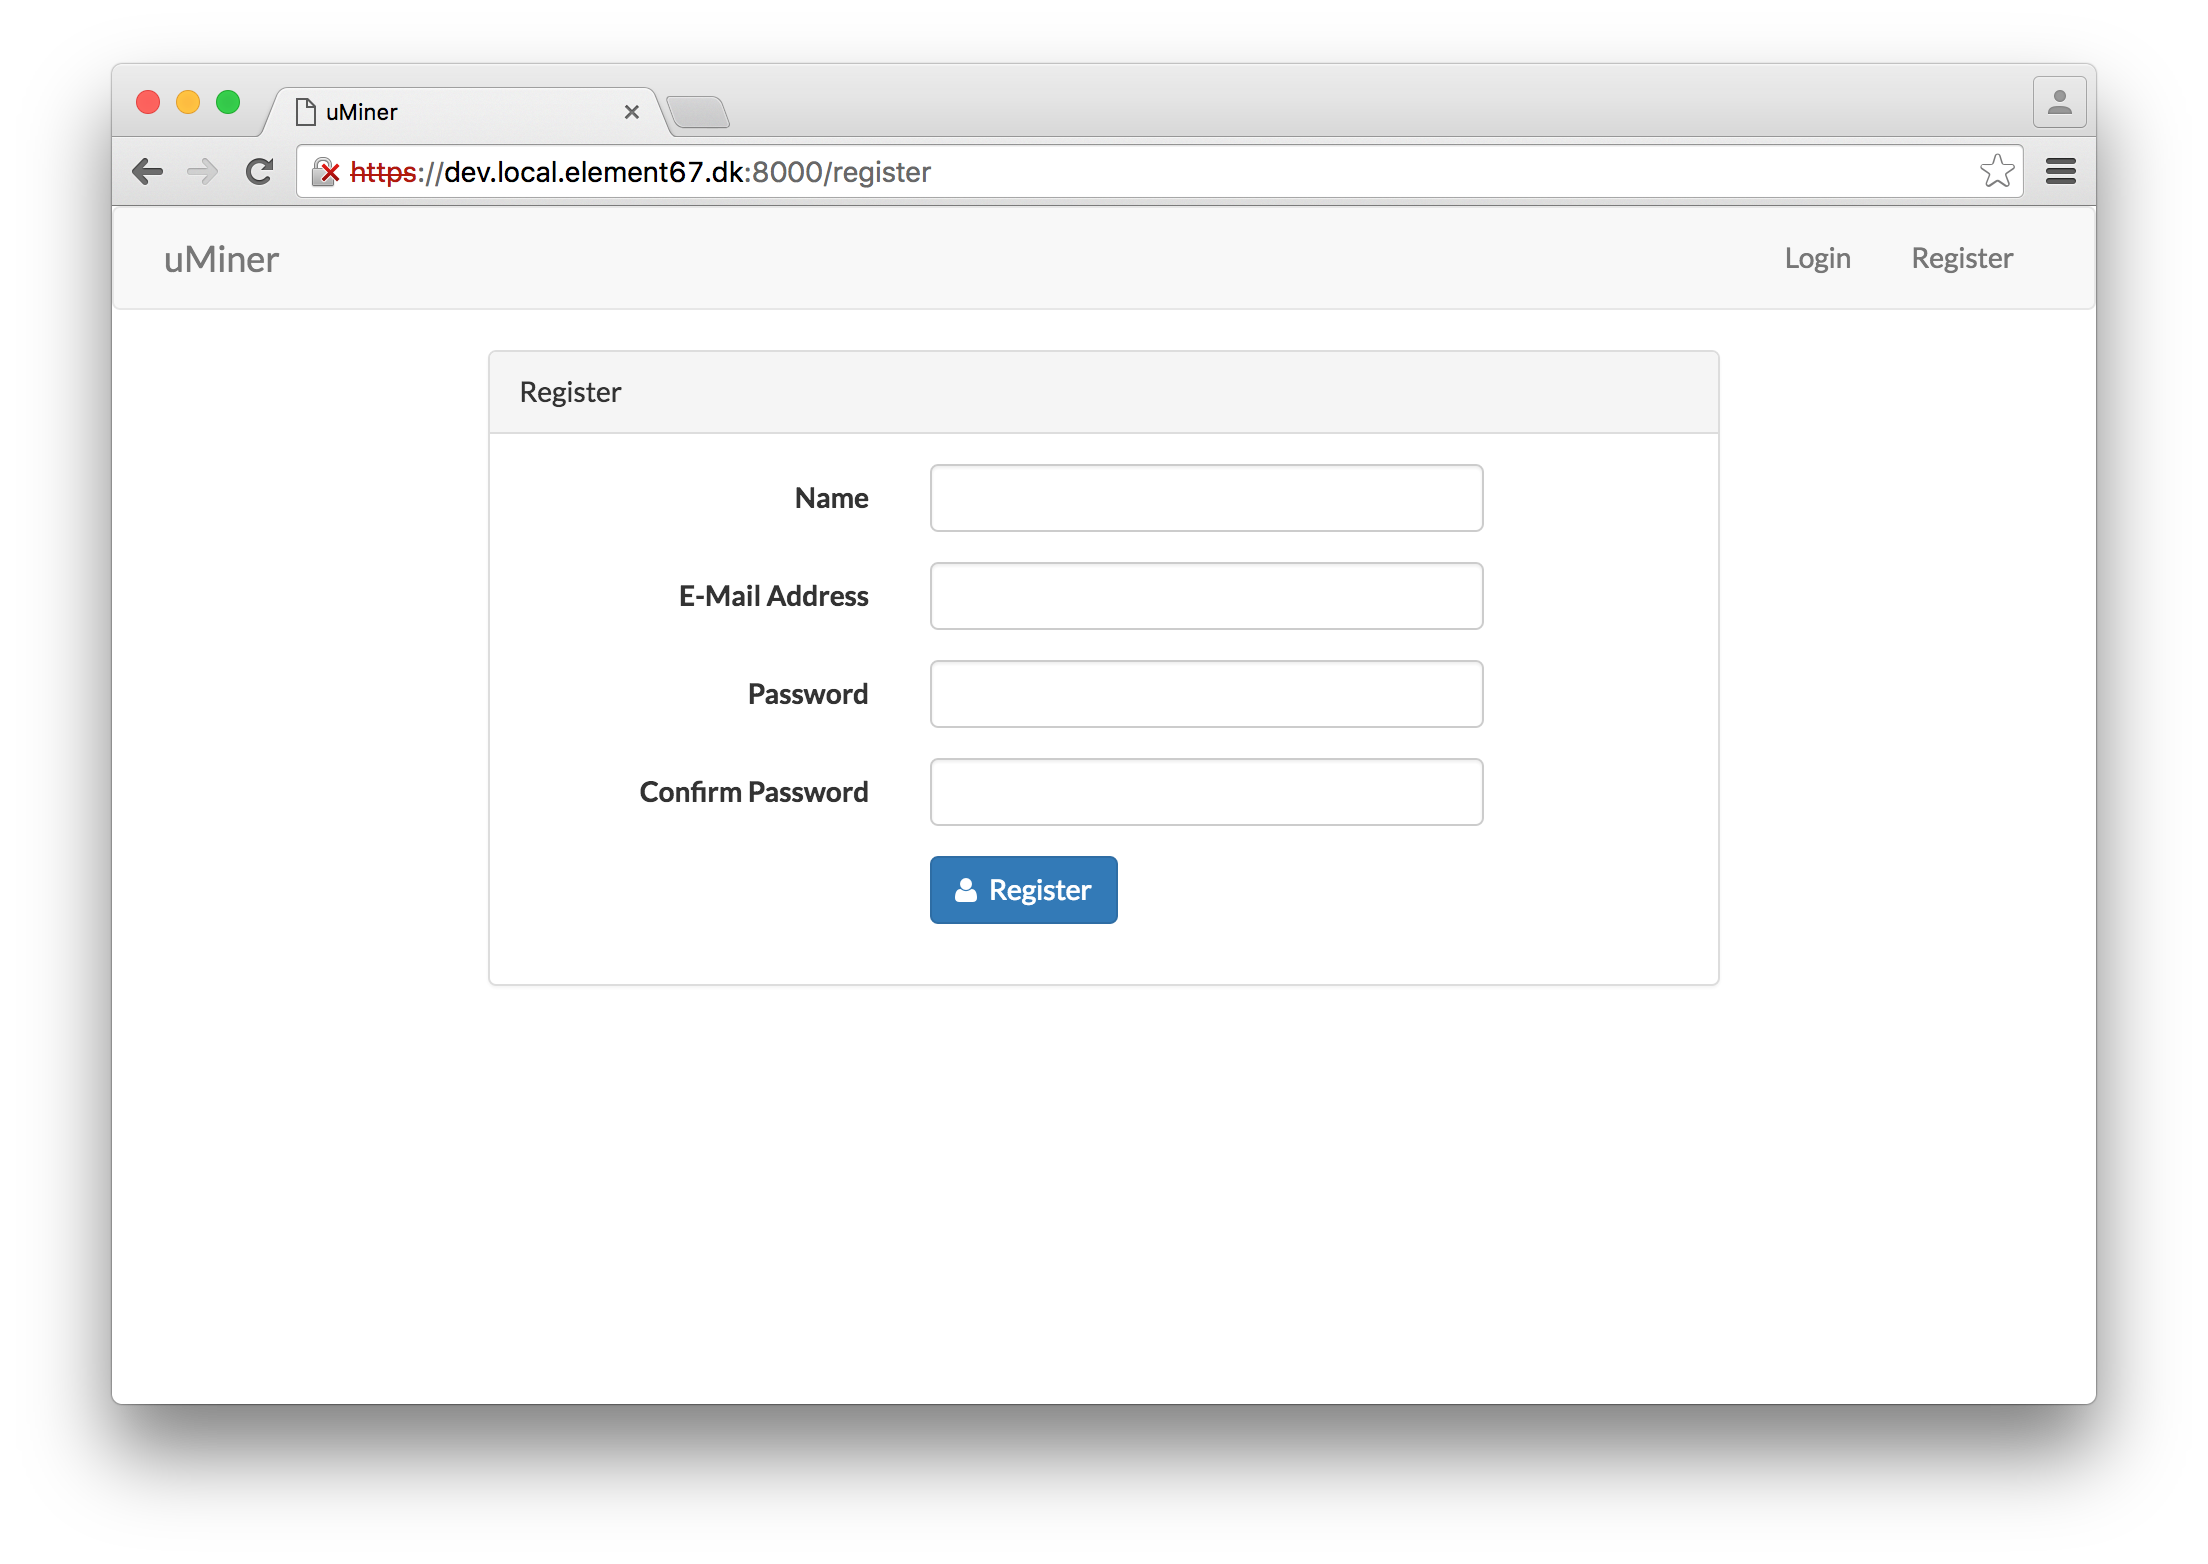
\includegraphics[width=\linewidth]{user_interfaces/web/web_register}
\caption{Register page.}
\label{fig:web_register}
\end{figure}
\FloatBarrier

% Login
\begin{figure}[!htbp]
\centering
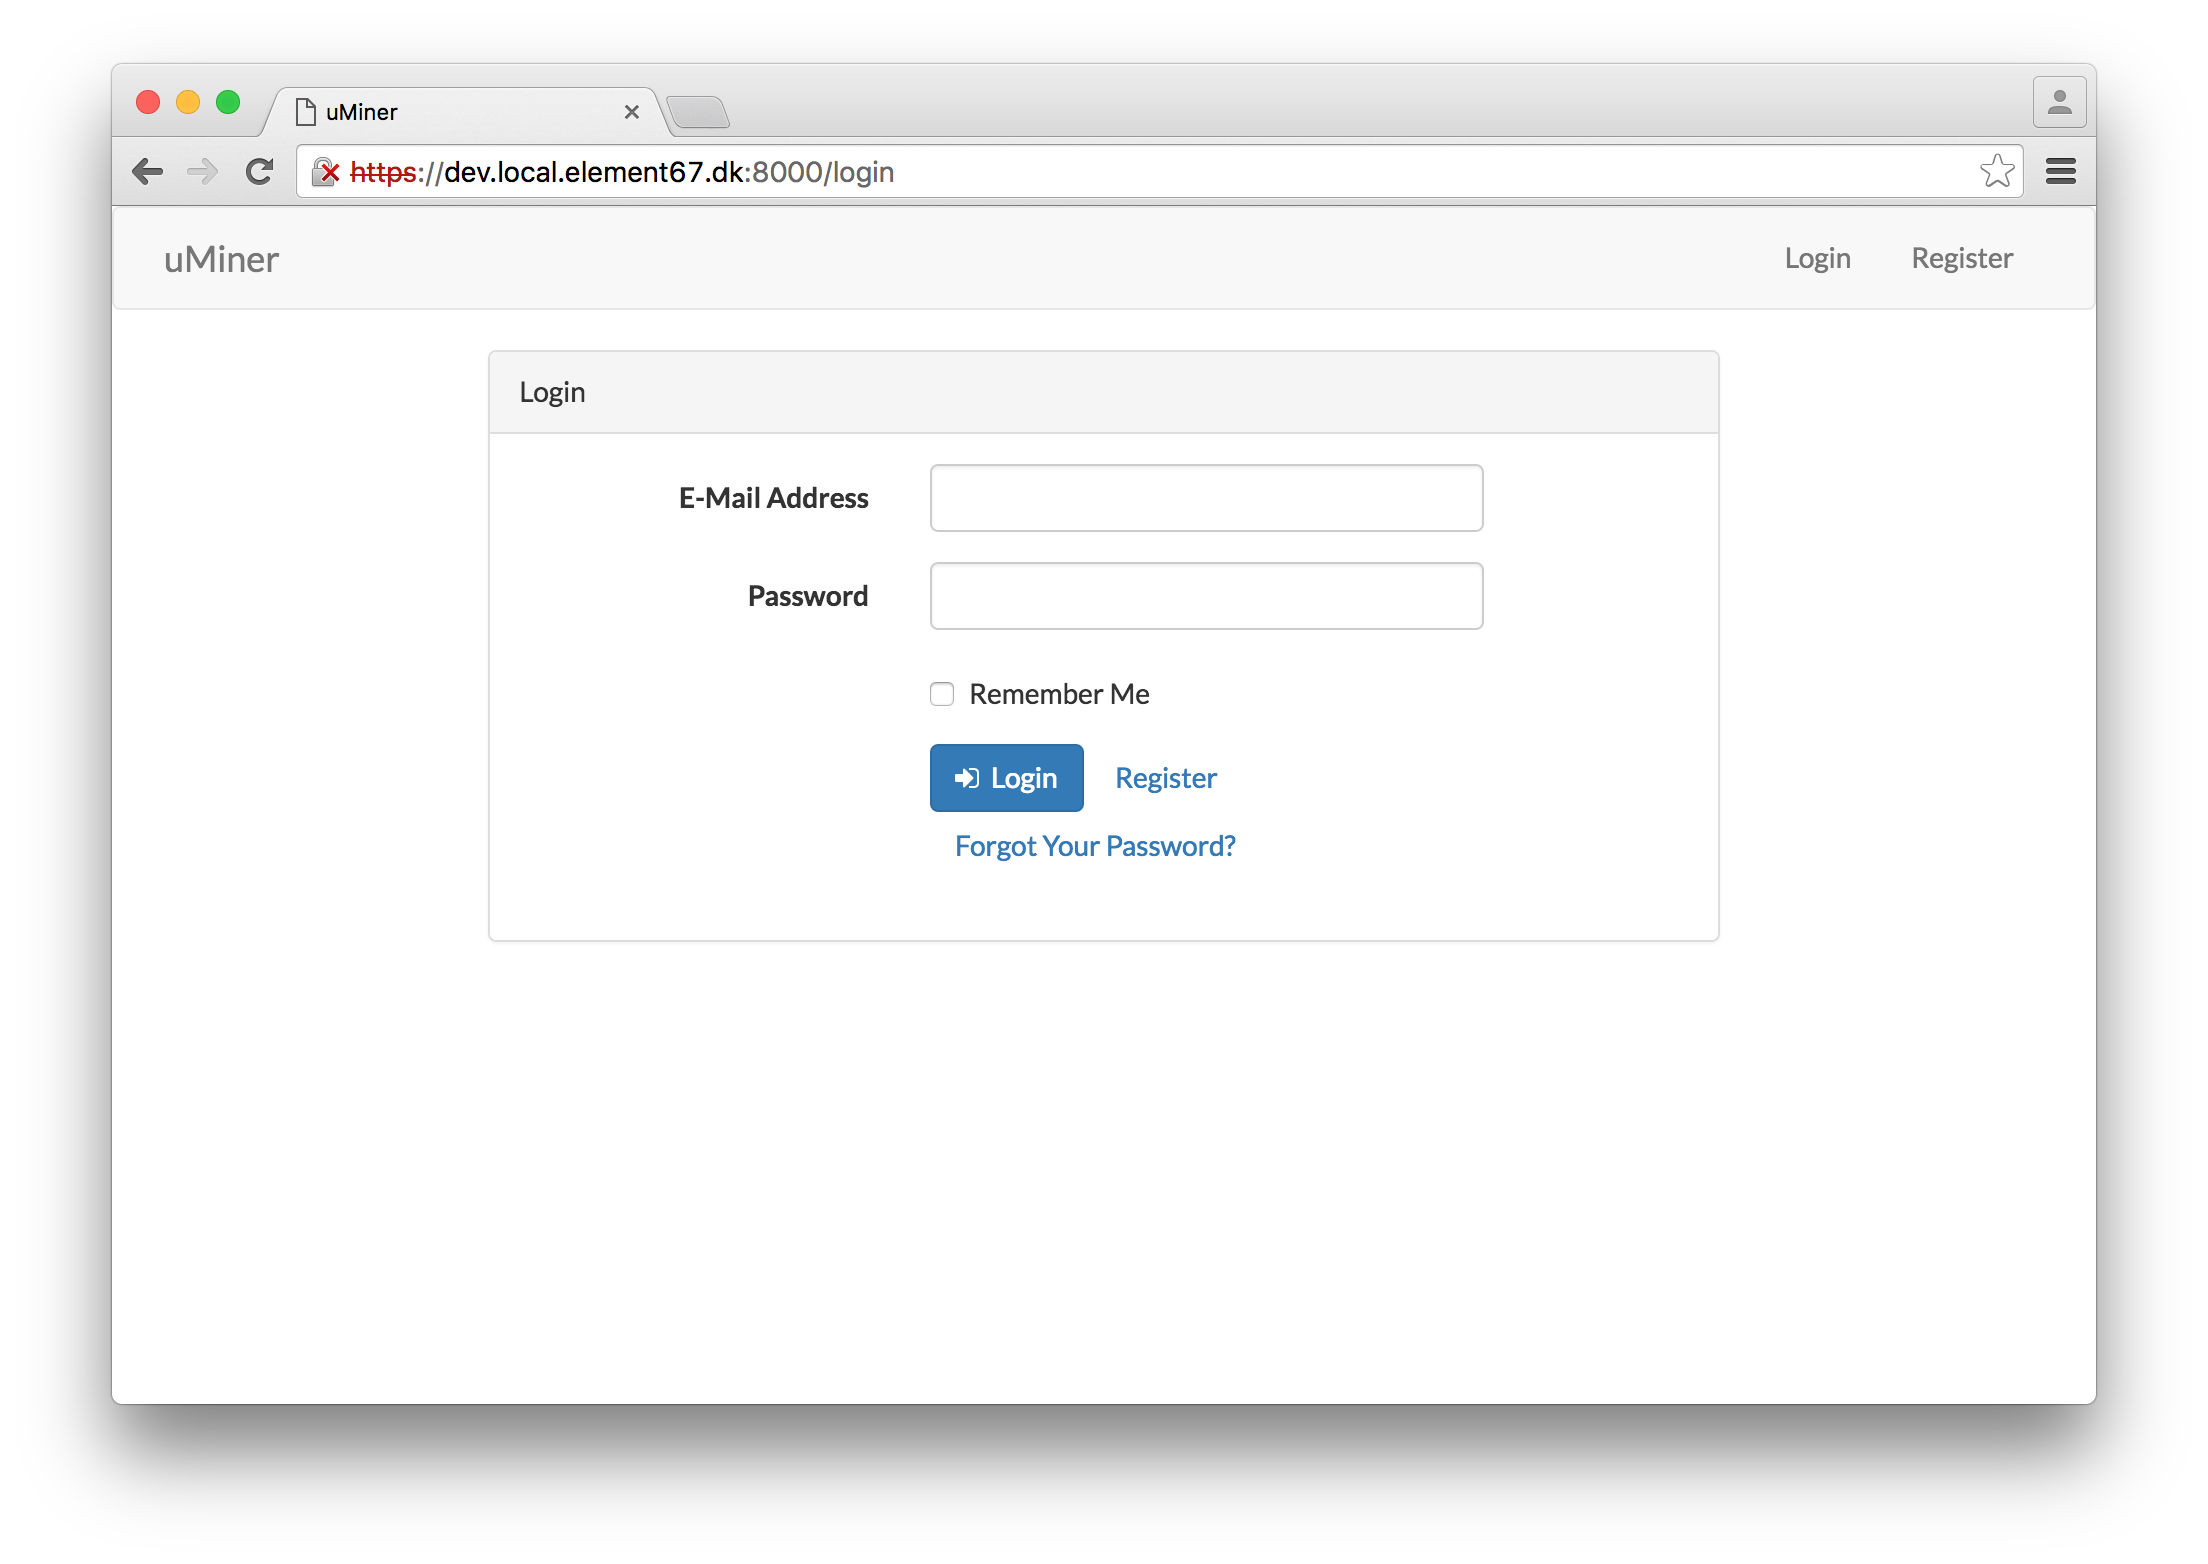
\includegraphics[width=\linewidth]{user_interfaces/web/web_login}
\caption{Log in page.}
\label{fig:web_login}
\end{figure}
\FloatBarrier

\subsection{Creating Campaign}

% Create campaign
\begin{figure}[!htbp]
\centering
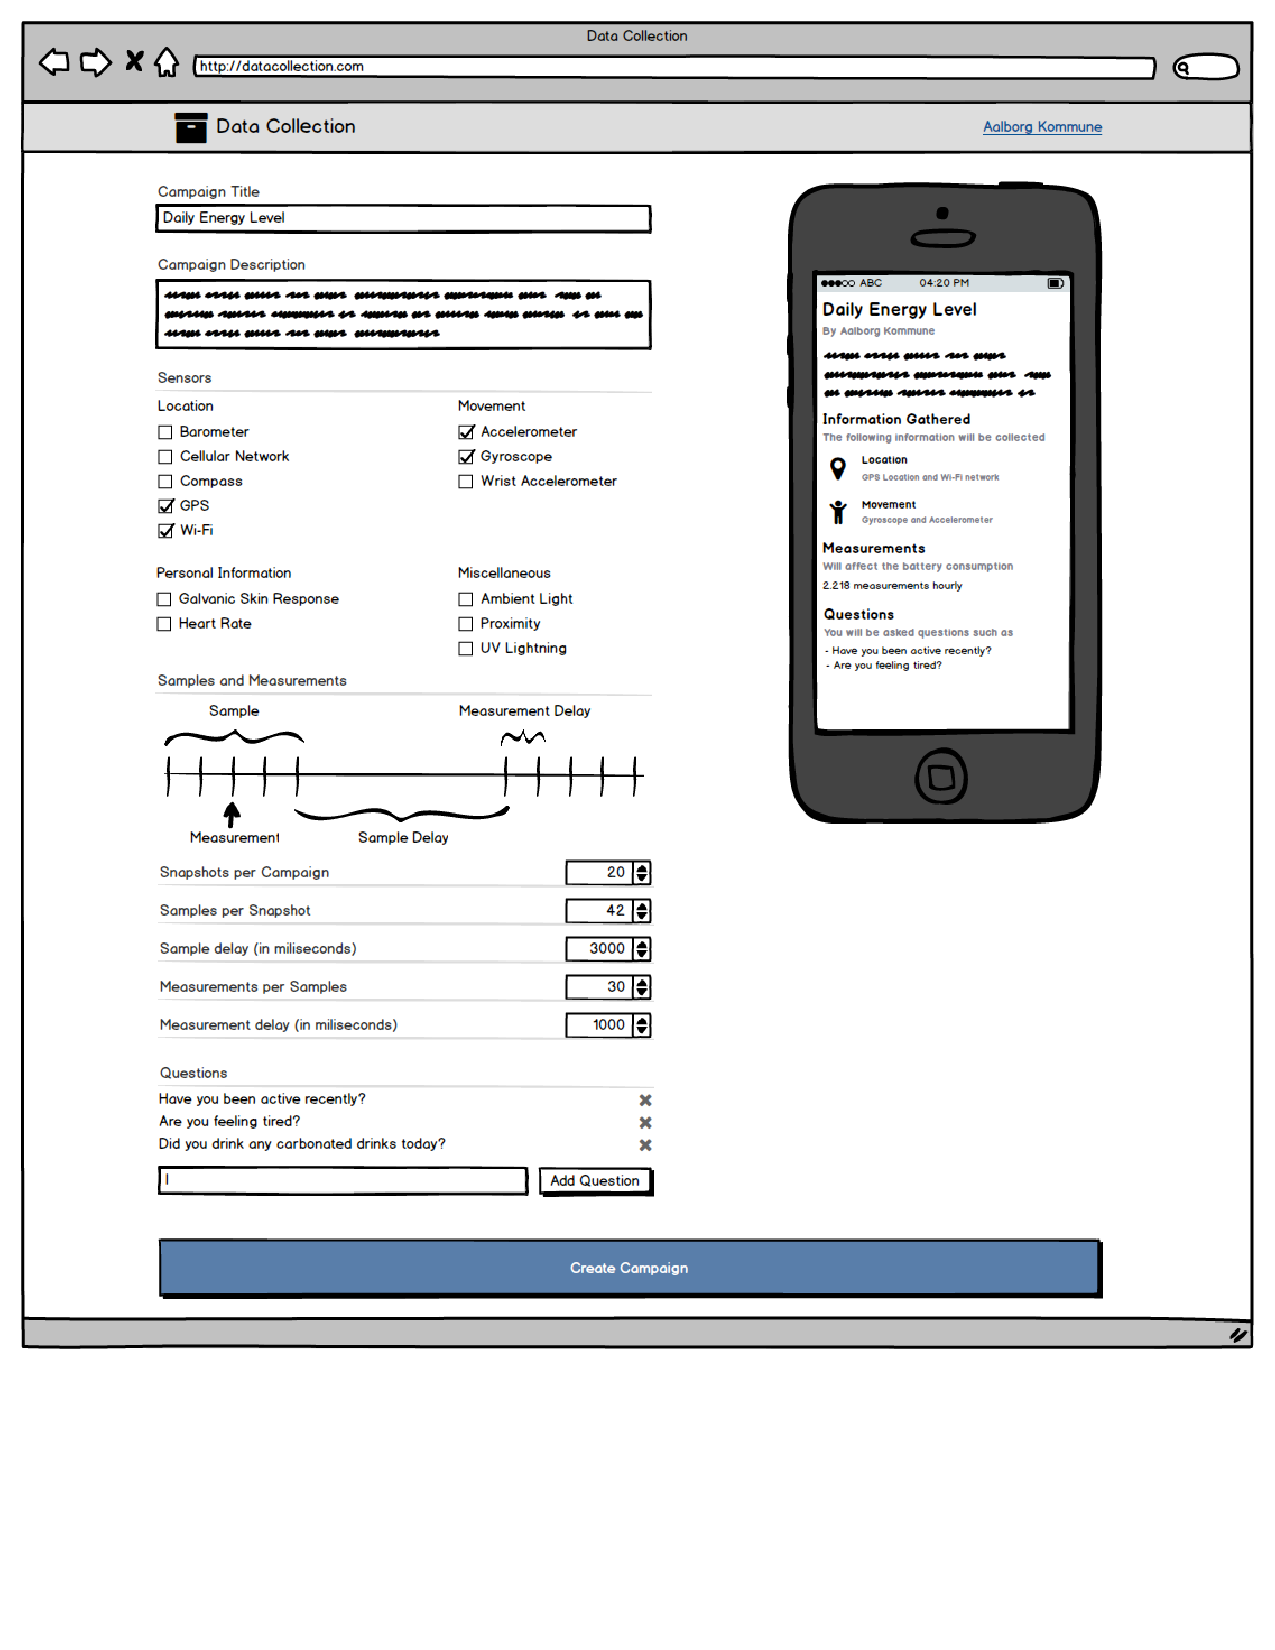
\includegraphics[width=\linewidth]{user_interfaces/web/web_create_campaign}
\caption{Creating Campaigns.}
\label{fig:web_create_campaign}
\end{figure}
\FloatBarrier

% View campaign
\begin{figure}[!htbp]
\centering
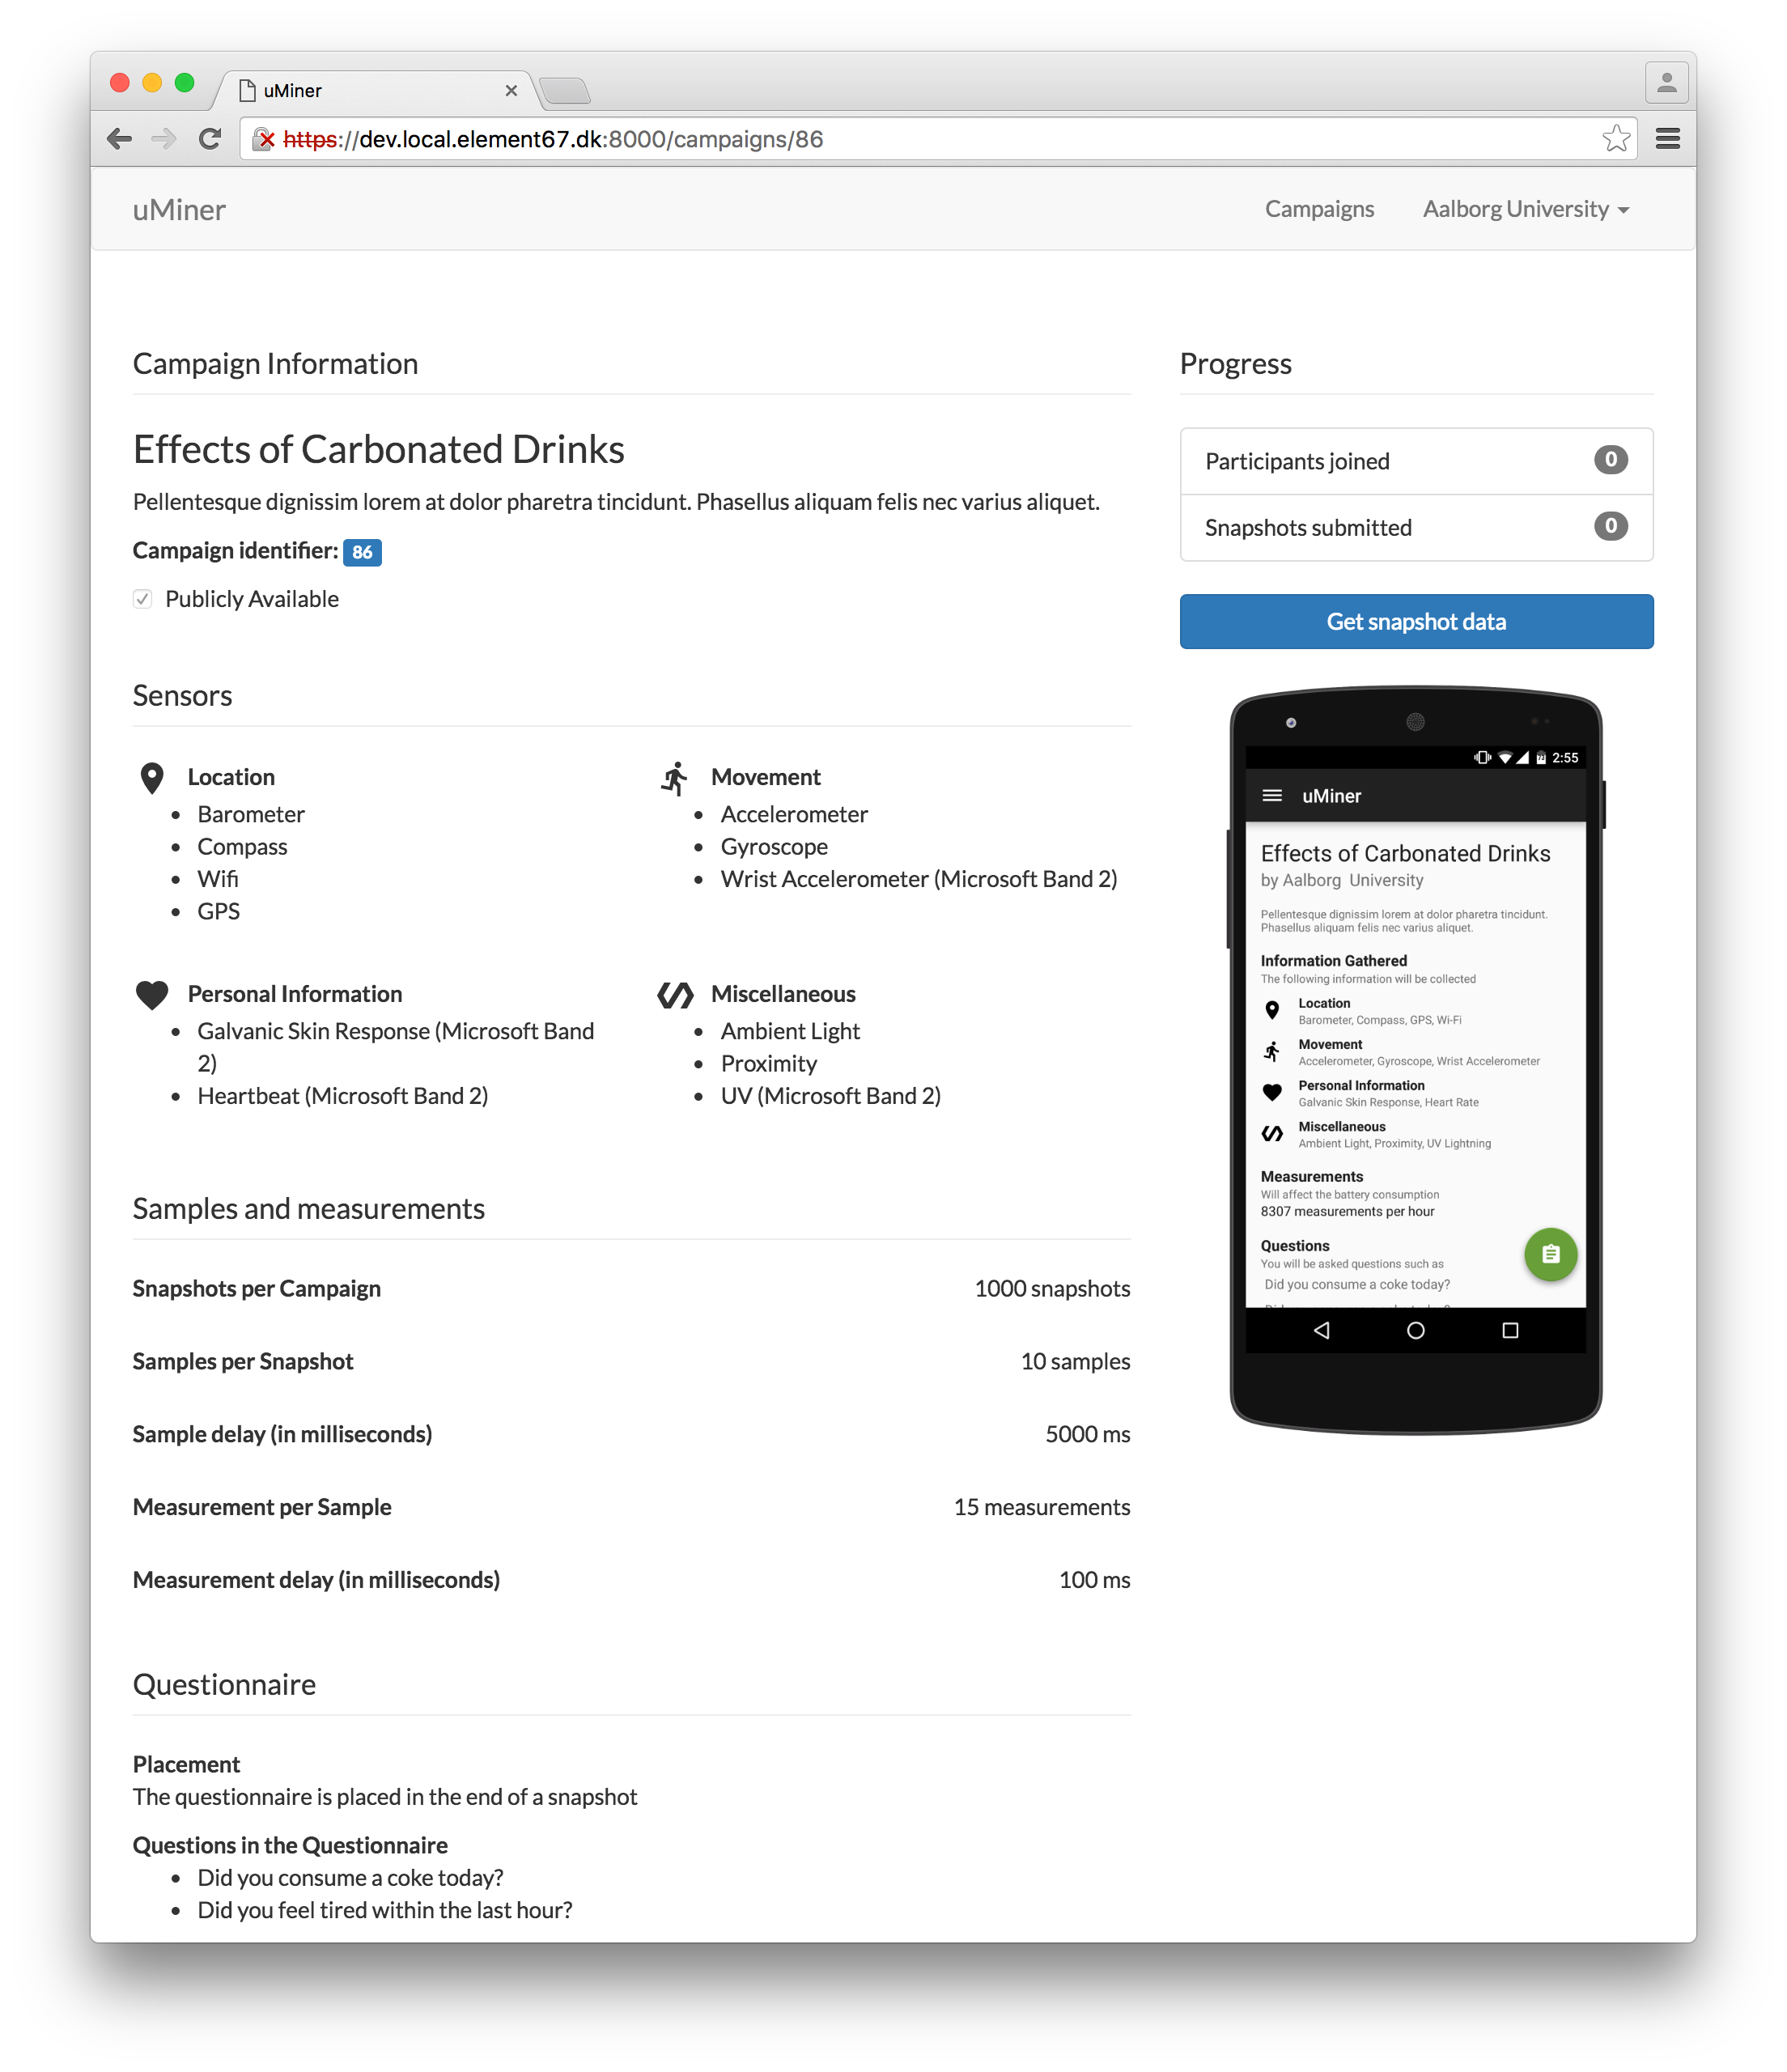
\includegraphics[width=\linewidth]{user_interfaces/web/web_view_campaign}
\caption{Viewing Campaigns.}
\label{fig:web_view_campaign}
\end{figure}
\FloatBarrier